\chapter{Zustandsautomat}

\section{Definition}

Ein endlicher Zustandsautomat kann im Allgemeinen als 5-Tupel dargestellt werden. Seine Form, $A=(Q, \Sigma, \delta, q_0, F)$, beinhaltet die Elemente:

$Q$ \quad endliche Menge aller Zust\"ande

$\Sigma$ \quad Eingabealphabet

$\delta: Q x \Sigma \rightarrow Q$ \quad \"Ubergangsfunktion

$q_0 \in  Q$ \quad Startzustand

$F \subseteq Q$ \quad Endzust\"ande

Hierbei ist die \"Ubergangsfunktion eine Funktion, mit der man von einem Zustand der Menge $Q$ \"uber eine definierte Eingabe der Menge $\Sigma$ zu einem weiteren Zustand der Menge $Q$ gelangt. Der Startzustand dient als Einstiegspunkt des Automaten. Jeder Automat besitzt weiterhin mindestens einen Endzustand, auch akzeptierender Zustand genannt. Sollte durch passende Eingabe ein solcher Zustand erreicht werden, so kann die Abarbeitung des Automaten enden.

\section{Deterministische und nichtdeterministische Zustandsautomaten}

Es gibt grunds\"atzlich zwei Arten der endlichen Zustandsautomaten. Ist es m\"oglich, das Ziel einer \"Ubergangsfunktion vollst\"andig vorherzusagen, d.h. kann durch Eingabe eines Symbols nur ein einziger Folgezustand erreicht werden, so spricht man von einem deterministischen Automaten. Im Gegensatz zu einem deterministischen Automaten k\"onnen bei einem nichtdeterministischen Automaten also bei Eingabe eines Symbols mehrere Zust\"ande erreicht werden, daher ist das Verhalten dieses Automaten nicht vorhersagbar. Da der Umgang mit nichtdeterministischen Automaten \"außerst kritisch ist und jeder nicht deterministische Automat in einen \"aquivalenten deterministischen Automaten umgewandelt werden kann, wird im Folgenden der Algoritmus zur Umwandlung eines nichtdeterministischen Automaten in einen deterministischen Automaten vorgestellt.

Zur Umwandlung der Automaten wurde der Algorithmus der Potenzmengenkonstruktion verwendet. Hierbei wird eine Tabelle erstellt, in der ersichtlich ist, \"uber welche Eingaben welche Zust\"ande erreicht werden k\"onnen. Begonnen wird dabei im Startzustand des Automaten. F\"ur jede neue Kombination aus Zielzust\"anden wird nun ein neuer Zustand erzeugt und f\"ur diesen die Zielzust\"ande \"uberpr\"uft, bis sich keine neuen Kombinationen ergeben. Der neue Automat kann nun einfach aus der Tabelle abgelesen werden, wie in folgender Abbildung ersichtlich.

\begin{figure}[h]
 \centering
 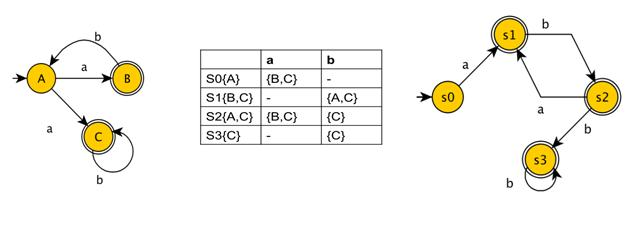
\includegraphics[keepaspectratio, scale=0.89]{objectsToInclude/Potenzmengenkonstruktion.jpg}
 \caption{Beispiel zur Potenzmengenkonstruktion}
\label{fig:FSA_PMK}
\end{figure}

\section{Datenstruktur} 

Endliche Zustandsautomaten (FSA) werden in diesem Projekt als Listen von States (Zust\"anden) und Transitionen (\"Ubergangsfunktionen) aufgebaut. Eine gesonderte Reihenfolge der Elemente einer Liste ist hierbei nicht zu beachten, da die Struktur des Automaten durch die einzelnen Transitionen abgebildet wird.

\section{Implementation}
Die Klasse FiniteStateAutomaton besitzt zwei Listen bzw. Vektoren, die TransitionList und die StateList, durch welche die Abbildung eines kompletten Automaten m\"oglich ist.

Die TransitionList setzt sich aus Elementen der Klasse Transition zusammen. Diese Elemente wiederum bestehen aus zwei Pointern, welche auf Elemente der Klasse State zeigen, sowie dem f\"ur den \"Ubergang zust\"andigen Eingabesymbol, welches als Text in der String-Variablen szEdge gespeichert ist.

Die Elemente der Klasse State, welche in der StateList gespeichert werden, enthalten eine String-Variable szName und zwei Boolean-Variablen, welche angeben, ob der State entweder ein Startzustand (bStartState) oder ein Endzustand (bFinalState) ist. Nat\"urlich kann ein State gleichzeitig Start- als auch Endzustand sein.

\section{Einlesen von endlichen Zustandsautomaten}

Das Einlesen eines endlichen Zustandsautomaten aus einer Textdatei ist als Funktion der Klasse FiniteStateAutomaton realisiert, selbiges gilt für das Schreiben in eine Textdatei. Beim Aufruf der Funktionen $write$ und $read$ ist jeweils der Name der Textdatei, aus der gelesen oder in die geschrieben werden soll, in Stringform zu \"ubergeben.

Das Einlesen und Schreiben erfolgt Zeilenweise und ist so strukturiert, dass die Objekte durch ihre Entsprechenden Tags gekapselt sind. Beispielhaft ist diese Darstellung im Folgenden für die States dargestellt:

<States> \\
State1 \\
State2 \\
</States>

Diese Art der Darstellung erm\"oglicht einen inhomogenen Aufbau der Textdatei, so dass es mehrere Bereiche geben kann, an denen States aufgef\"uhrt sind und sie trotzdem auch alle als solche erkannt werden.

Die Textdateien sind so aufgebaut, dass zuerst alle States, dann der StartState und zum Schluss alle Transitionen ausgegeben werden.

\section{Konvertierung}

\begin{figure}[h]
 \centering
 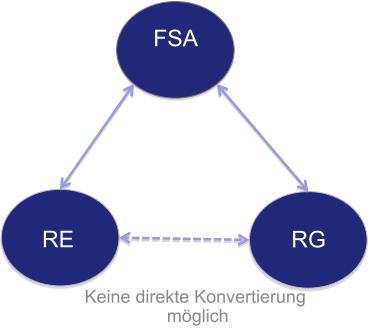
\includegraphics[keepaspectratio, scale=0.89]{objectsToInclude/Konvertierung.jpg}
 \caption{Konvertierungen}
\label{fig:FSA_Konv}
\end{figure}

Die Konvertierungen zwischen regul\"arem Ausdruck und endlichem Zustandsautomat, sowie regul\"arer Grammatik und endlichem Zustandsautomaten, sind direkt m\"oglich. Bei der Konvertierung zwischen regul\"arem Ausdruck und regul\"arer Grammatik muss man einen Umweg \"uber den endlichen Zustandsautomaten in  Kauf nehmen.

\section{Minimierung nach dem Moore-Algorithmus}

Bei der Minimalisierung nach dem Moore Algorithmus werden zuerst alle States in accepting und rejecting States unterteilt. Accepting sind all diejenigen, die ein Endzustand sind und rejecting alle anderen. Von nun  an werden diese beiden Bereiche getrennt behandelt.

Das Vorgehen ist nun wie folgt. Man stelle eine Tabelle auf, die auf der Vertikalen alle m\"oglichen Eingaben enth\"alt. Dann trage man auf der Horizontalen zwei Gruppen auf. Die eine Gruppe enth\"alt die Namen aller rejecting States (im folgenden Beispiel G\_0 der ersten Zeile), die andere enthält die Namen aller accepting States (im folgenden Beispiel G\_1 der ersten Zeile). Nun f\"ulle man die Elemente der Tabelle, indem man zu jeder Eingabe und jedem Statename angibt, welche Gruppe das Resultat der Transition aus gegebenem State und Eingabe w\"are, \"ahnlich der Vorgehensweise in der Potenzmengenkonstruktion.
 
Sind alle Elemente ausgef\"ullt, so beginnt man neue Gruppen zu erstellen. Daf\"ur wird wie folgt vorgegangen: Man vergleicht die Elemente, die unter einem State aufgelistet sind, mit den Elementen, die unter den Nachbarstates der gleichen Ausgangsgruppe aufgelistet sind. Haben alle States einer Ausgangsgruppe f\"ur die jeweilige Eingabe die gleiche Folgegruppe, so ist die Ausgangsgruppe minimal. Gibt es jedoch einen State, der f\"ur die gleiche Eingabe eine andere Folgegruppe hat, so wird eine neue Gruppe erstellt und der State in diese Gruppe verschoben.

Dieser Ablauf wiederholt sich so lange, bis alle Gruppen minimal sind. Die minimalen Gruppen entsprechen abschließend dann den States des minimalisierten endlichen Automaten. Das folgende Beispiel beschreibt diesen Vorgang nochmal beispielhaft:

\begin{figure}[h]
 \centering
 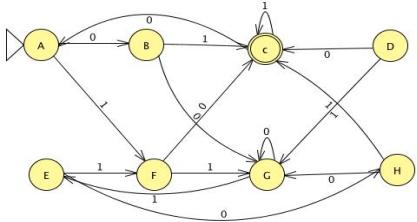
\includegraphics[keepaspectratio, scale=0.75]{objectsToInclude/Moore_nichtminimal.jpg}
 \caption{Nicht minimierter Automat}
\label{fig:FSA_Moore_notminimal}
\end{figure}

\begin{figure}[h]
 \centering
 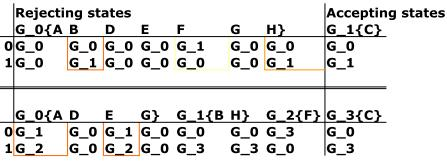
\includegraphics[keepaspectratio, scale=0.75]{objectsToInclude/Moore_Tab.jpg}
 \caption{Tabelle zum Minimierungsvorgang}
\label{fig:FSA_Moore_Tab}
\end{figure}

\begin{figure}[h]
 \centering
 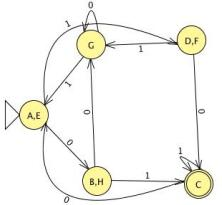
\includegraphics[keepaspectratio, scale=0.75]{objectsToInclude/Moore_minimal.jpg}
 \caption{Resultierender minimierter Automat}
\label{fig:FSA_Moore_minimal}
\end{figure}
